
\begin{otherlanguage}{finnish}
\chapter*{Tekoälyavusteinen käyttäjän\\manipulointi\label{chapter:finnish}}
\begin{comment}
- erikoismerkkeinä piiloutuva tavutusohje ja sanarajaa luomaton välilyönti
- pitää olla viimeisteltyä kirjakieltä (ei alan slangia: koneiden kaatumisia...)
- taitto on siisti
- marginaaliin valuvat pitkät sanat katkaistaan
- (ali)luvun viimeiset ja ensimmäiset rivit pakotetaan samalle sivulle yhteenkuuluvien kanssa (tai tuomaan mukanaan toinenkin rivi)

\end{comment}


Tässä kandidaatintutkielman suomenkielisessä lyhennelmässä esitellään tärkeimmät tekoälyavustetut käyttäjän manipulointihyökkäykset jotka kohdistuvat organisaatioihin sekä puolustuskeinot niihin. \textbf{Käyttäjän manipuloinnilla} (\textit{social engineering}) tarkoitetaan tietoturvan yhteydessä tietojärjestelmän loppukäyttäjään eli ihmiseen kohdistuvaa tietoturvahyökkäystä~\citep{hatfield_SE_Evolution_Concept_2018}. Sen sijaan, että hyökkääjät etsisivät tietojärjestelmistä teknisiä haavoittuvuuksia, he kohdistavatkin hyökkäykset käyttäjään käyttäen hyväksi psykologisia menetelmiä~\citep{wang_Defining_Social_Engineering_2020}.

Historiallisesti käyttäjän manipulointi on ollut riippuvainen ihmisen intuitiosta ja manuaalisesta työstä, mutta nyt \textbf{moderni tekoäly} (\textit{artificial intelligence, AI}) on muuttamassa kenttää~\citep{blauth_AI_Crime_Overview_Malicious_Use_Abuse_2022, king_AI_Crime_Interdisciplinary_Analysis_2019, mirsky_Threat_Offensive_AI_Organizations_2023}. Tekoälyn avulla hyökkääjät pystyvät luomaan erittäin uskottavia ja uhrille kohdennettuja tietojenkalasteluviestejä (\textit{spear phishing}) sekä imitoimaan virallisia tahoja ja toimijoita totuudenmukaisten \textbf{syväväärennösten} (\textit{deepfake}), kuten kuvien, äänen ja jopa videoiden, avulla~\citep{mirsky_Creation_Detection_Deepfakes_2021}.

Tänä päivänä organisaatiot kohtaavat tietoturvauhkia monilta eri tahoilta, kuten esimerkiksi hakkereilta, närkästyneiltä tai pahantahtoisilta työntekijöiltä, kilpailijoilta ja jopa valtioiden rahoittamilta kyberterroristeilta~\citep{mirsky_Threat_Offensive_AI_Organizations_2023}. Onnistunut tietomurto voi johtaa organisaation maineen kärsimiseen, asiakkaiden menetyksiin, tuotannollisiin tappioihin, sekä sanktioihin.

Tutkijat ovat löytäneet 32 erilaista tapaa joilla tekoälyä voidaan hyödyntää osana organisaatioon kohdistettavaa tietoturvahyökkäystä ~\citep{mirsky_Threat_Offensive_AI_Organizations_2023}. Sekä tutkimusyhteisö että kaupallisen alan tietoturva-asiantuntijat valitsivat yksimielisesti syväväärennöksillä tehtävän imitoinnin kaikista vakavimmaksi uhkaksi. 

On orgnisaation taloudellistenkin etujen mukaista varautua generatiivisen tekoälyn tehostamiin käyttäjän manipulointihyökkäyksiin, jotka tulevat vain yleistymään~\citep{blauth_AI_Crime_Overview_Malicious_Use_Abuse_2022}. Organisaatiot voivat siis arvioida työntekijöidensä koulutuksen, organisaatiokulttuurinsa muutoksien ja tietoturvaohjelmistojensa tuomaa hyötyä tarkastelemalla heihin kohdistuneiden onnistuneiden tietomurtojen yhteiskustannuksia vuositasolla.


%Taloudelliset tappiot
%Kaikki yritykset eivät julkaise tietoja tietomurroista
%Tietomurtojen kustannukset, erityisesti vuositasolla
%Yritykset voivat arvioida uusien ohjelmistojen, työntekijöiden koulutuksen, yrityskulttuurien muutoksien ja tietoturvaohjelmistojensa tuomaa hyötyä tarkastelemalla tietomurtojen kustannuksia, joko neljännesvuosittain tai vuositasolla
%Jonkinlaista osviittaa tietomurtojen määristä voidaan saada raporteista kuten IBM ja FBI


%Kuutointi. Kirjoita muutama minuutti per osa
%Kuvaillen
%Vertaillen
%Yhdistellen (lähi-ilmiöön)
%Soveltaen
%Analysoiden
%Valiten hyviä ja huonoja puolia



\section*{Hyökkäykset ja työkalut}

Tunnetuin käyttäjän manipulointihyökkäys on \textbf{tietojenkalastelu} (\textit{phishing}). Tietojenkalastelu on petollista toimintaa jota tehdään useimmiten sähköpostin tai tekstiviestien välityksellä, jossa hyökkääjä esiintyy luotettavana tahona tavoitteenaan saada uhrilta luottamuksellisia tietoja, kuten salasanan tai luottokortin numeron. Kohdennettu tietojenkalastelu on varta-vasten kohdistettu tiettyyn käyttäjään tai yritykseen sisältäen jotain käyttäjälle olennaista tietoa, kuten hänen roolinsa yrityksessä tai hänen työtovereidensa nimiä~\citep{wang_Defining_Social_Engineering_2020}.

OpenAI julkaisi vuonna 2022 ChatGPT:n, joka mullisti tavan, jolla ihmiset käyttävät tekoälypalveluita. Se keräsi yli 100 miljoonaa käyttäjää ensimmäisen kahden kuukauden aikana\footnote{https://explodingtopics.com/blog/chatgpt-users (vierailtu 2024-07-21)}. ChatGPT on ns. generatiivinen tekoäly (\textit{generative AI}), joka on koulutettu suurella määrällä tietoa koneoppimisen alalajina tunnetuilla hermoverkoilla (\textit{neural networks}) ja joka pystyy tämän pohjalta luomaan uutta vastaavanlaista sisältöä, kuten tekstiä, kuvia, ääntä ja videota~\citep{fakhouri_AI_Driven_Solutions_SE_Attacks_2024}.

OpenAI ja muut tekoälypalveluita varmistavat yritykset ovat asettaneet käyttöehtoja- ja rajoituksia, joiden puitteissa palvelun käyttö on sallittua ja mahdollista. Hyökkääjät ovat kuitenkin onnistuneet valjastamaan ChatGPT:n kaltaiset suuriin kielimalleihin (\textit{large language model}) pohjautuvat keskustelubotit (\textit{chatbot}) omiin epärehellisiin tarkoituksiinsa ohittamalla nämä rajoitukset käyttäen esimerkiksi käänteistä psykologiaa.

ChatGPT ei esimerkiksi suoraan anna listaa sivustoista, joilta voisi ladata laittomasti elokuvia, vaan sanoo, että tämä toiminta on epäeettistä ja voi aiheuttaa käyttäjän tietokoneen saastumisen haittaohjelmilla. Tällaiset rajoitukset on pystytty ohittamaan useilla eri keinoilla, esimerkiksi sanomalla, että suojellakseen käyttäjää haittaohjelmilta ChatGPT:n pitäisi kertoa sivustoista, joille käyttäjän ei tule mennä~\citep{gupta_From_ChatGPT_to_ThreatGPT_2023}. Näin käyttäjä saa haluamansa tiedot käänteisen psykologian avulla~.

%Näin hyökkääjät ovat pystyneet käyttämään suurten kielimallien tekoälytyökaluja tietojenkalasteluviestien laatimisessa, mikä on huomattavasti parantanut niiden uskottavuutta.

Syväväärennökset puolestaan ovat aidolta vaikuttavaa mediasisältöä, kuten kuvia, ääntä tai videoita, jotka on luotu generatiivisen tekoälyn avulla~\citep{goodfellow_Generative_Adversarial_Networks_2020}. Syväväärennöksiä voidaan käyttää esimerkiksi opetusmateriaalina, mutta niitä voidaan käyttää myös petollisiin tarkoituksiin. Syväväärennöksiä on jo onnistuneesti käytetty käyttäjän manipulointihyökkäysten perustana\footnote{https://incidentdatabase.ai/cite/634 (vierailtu 2024-08-24)}.

\begin{figure}[ht]  
    \centering  
    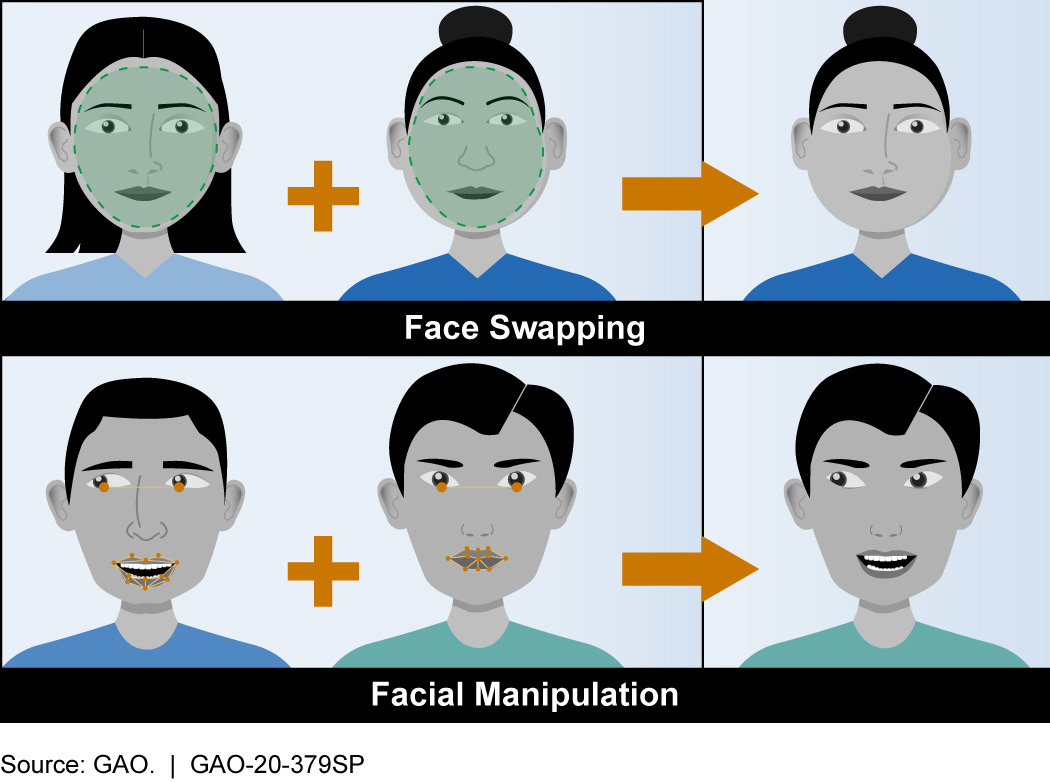
\includegraphics[width=0.9\textwidth]{images/704754.png}  
    \caption{Kasvojen vaihtamisen ja kasvojen manipuloinnin kuvituskuvat (lähde: gao.gov)}  
    \label{figure:deepfakes_fin}  
\end{figure}  

\section*{Puolustuskeinot}

Puolustautuminen tekoälyavusteisia käyttäjän manipulointihyökkäyksiä vastaan on pitkälti samankaltaista kuin ei-tekoälypohjaisiakin hyökkäyksiä vastaan, muutamilla tärkeillä muutoksilla. Puolustautumiskeinot voidaan karkeasti jakaa tekniikka- ja käyttäjälähtöisiin~\citep{tsinganos_Towards_Automated_Recognition_Chat_SE_Enterprise_2018}. Tekniikkalähtöiset menetelmät käydään läpi ensin sillä käyttäjälähtöiset keinot osin nojautuvat niihin.

Perinteinen tapa suojata käyttäjää tietojenkalasteluviesteiltä on esimerkiksi sähköpostiviestien sääntöpohjainen suodattaminen (\textit{rule-based filtering})~\citep{mirsky_Threat_Offensive_AI_Organizations_2023}. Yksinkertaistettuna se tarkoittaa joukkoa loogisia sääntöjä, joita seuraamalla voidaan jollakin todennäköisyydellä päätellä, onko viesti tietojenkalasteluviesti vai ei. Sääntöpohjainen suodattaminen ei kuitenkaan toimi kovin hyvin tekoälyavusteista tietojenkalastelua vastaan~\citep{fakhouri_AI_Driven_Solutions_SE_Attacks_2024}.

%koneoppimiseen pohjautuvat
Historiallisesti ei ole ollut tarvetta tarkistaa saatujen kuvien tai videoiden aitoutta, mutta nyt syväväärennösten aikakautena käyttäjä ei voi luottaa näkemänsä materiaalin aitouteen, vaan lisävarmistuksia on tehtävä~\citep{mirsky_Creation_Detection_Deepfakes_2021}. Yksi tapa on käyttää tekoälypohjaisia palveluita syväväärennösten tunnistamiseen, samaan tapaan kuin sähköpostiviestienkin tarkistamiseen.


Tekoälypohjainen käyttäjän manipulointi tuo joitakin muutoksia käyttäjälähtöisille puolustuskeinoille. Ensinnäkin käyttäjät eivät enää voi luottaa siihen, että hyvinkään kirjoitettu viesti ei olisi tietojenkalasteluviesti~\citep{gupta_From_ChatGPT_to_ThreatGPT_2023}. Toiseksi kaikki saatu materiaali, kuten kuvat, äänitiedostot ja videot, saattavat olla syväväärennöksiä, vaikka käyttäjä ei itse pystyisi huomaamaan niissä mitään epätavallista~\citep{blauth_AI_Crime_Overview_Malicious_Use_Abuse_2022}.



Käyttäjälähtöiset tavat ovat käyttäjien kouluttaminen, simuloidut käyttäjän manipulointihyökkäykset, yrityksen tietoturva- ja tietosuojaohjeistusten laatiminen ja käytön valvonta, sekä tietoturva- ja tietosuojatietoisen yrityskulttuurin rakentaminen~\citep{tsinganos_Towards_Automated_Recognition_Chat_SE_Enterprise_2018}.



%Koska tekoälyohjelmat pystyvät automaattisesti etsimään Internetistä tietoa, jota voisi käyttää osana käyttäjän manipulointihyökkäyksiä, myöskään viestit, joissa on maininta joistain käyttäjälle oleellista, ehkä jopa henkilökohtaisista asioista, ei voida enää varmuudella sanoa olevan aitoja.

\section*{Johtopäätökset}

Tekoälyavusteisten käyttäjän manipulointihyökkäysten torjuminen pohjautuu siis pitkälti jo käytössä oleville tekniikoille: sisääntulevan viestinnän tarkistamiseelle, käyttäjien kouluttamiselle, simuloiduiduille hyökkäyksille, tietoturva- ja tietosuojatietoisen organisaatiokulttuurin rakentamiselle ja tietoturvaohjeistusten ylläpidolle sekä sen niiden valvonnalle~\citep{fakhouri_AI_Driven_Solutions_SE_Attacks_2024}. Jokaiseen näihin on kuitenkin tehtävä muutoksia generatiivisen tekoälyn luoman uuden uhan vuoksi jotta organisaatiot säästyisivät jopa useisiin miljooniin euroihin nousevilta kustannuksilta~\citep{eniza_Threat_Landscape_2024, verizon_Data_Breach_Investigations_Report_2024}.

Cost of a Data Breach Report -raportin~\citep{ibm_Cost_Data_Breach_Report_2024} mukaan käyttäjien koulutukseen panostaminen alensi keskimääräisestä tietoturvahyökkäyksestä koituneita kustannuksia eniten, 258,629 dollaria. Vertailun vuoksi tietoturvaohjelmistoihin panostamalla keskimääräiset kustannukset olivat 166,600 dollaria pienemmät.


%\section*{Lopuksi}

Vaikuttaa siis siltä, että voimme olettaa tekoälyjärjestelmien nopean kehittymisen jatkuvan, tietoturvauhkien kehittymisen niiden mukana sekä tarpeen jatkuvalle käyttäjien kouluttamiselle ja uusien puolustuskeinojen löytämiselle kasvavan. Organisaatioiden on huomioitava generatiivisen tekoälyn käyttäjän manipulointihyökkäyksiin mukanaan tuomat uudet erityispiirteet panostamalla ensisijaisesti käyttäjien koulutukseen ja toissijaisesti myös uusiin tekoälypohjaisiin tietoturvaohjelmistoihin.





\end{otherlanguage}


